\section{Partie 1 \label{sec:partie_1}}

\subsection{Partie 1.1} % On peut aussi mettre le label juste en dessous
\label{sec:partie_1_1}

\subsubsection{Partie 1.1.1}

\autoref{fig:chat1}

\begin{figure}[ht]
	\centering
	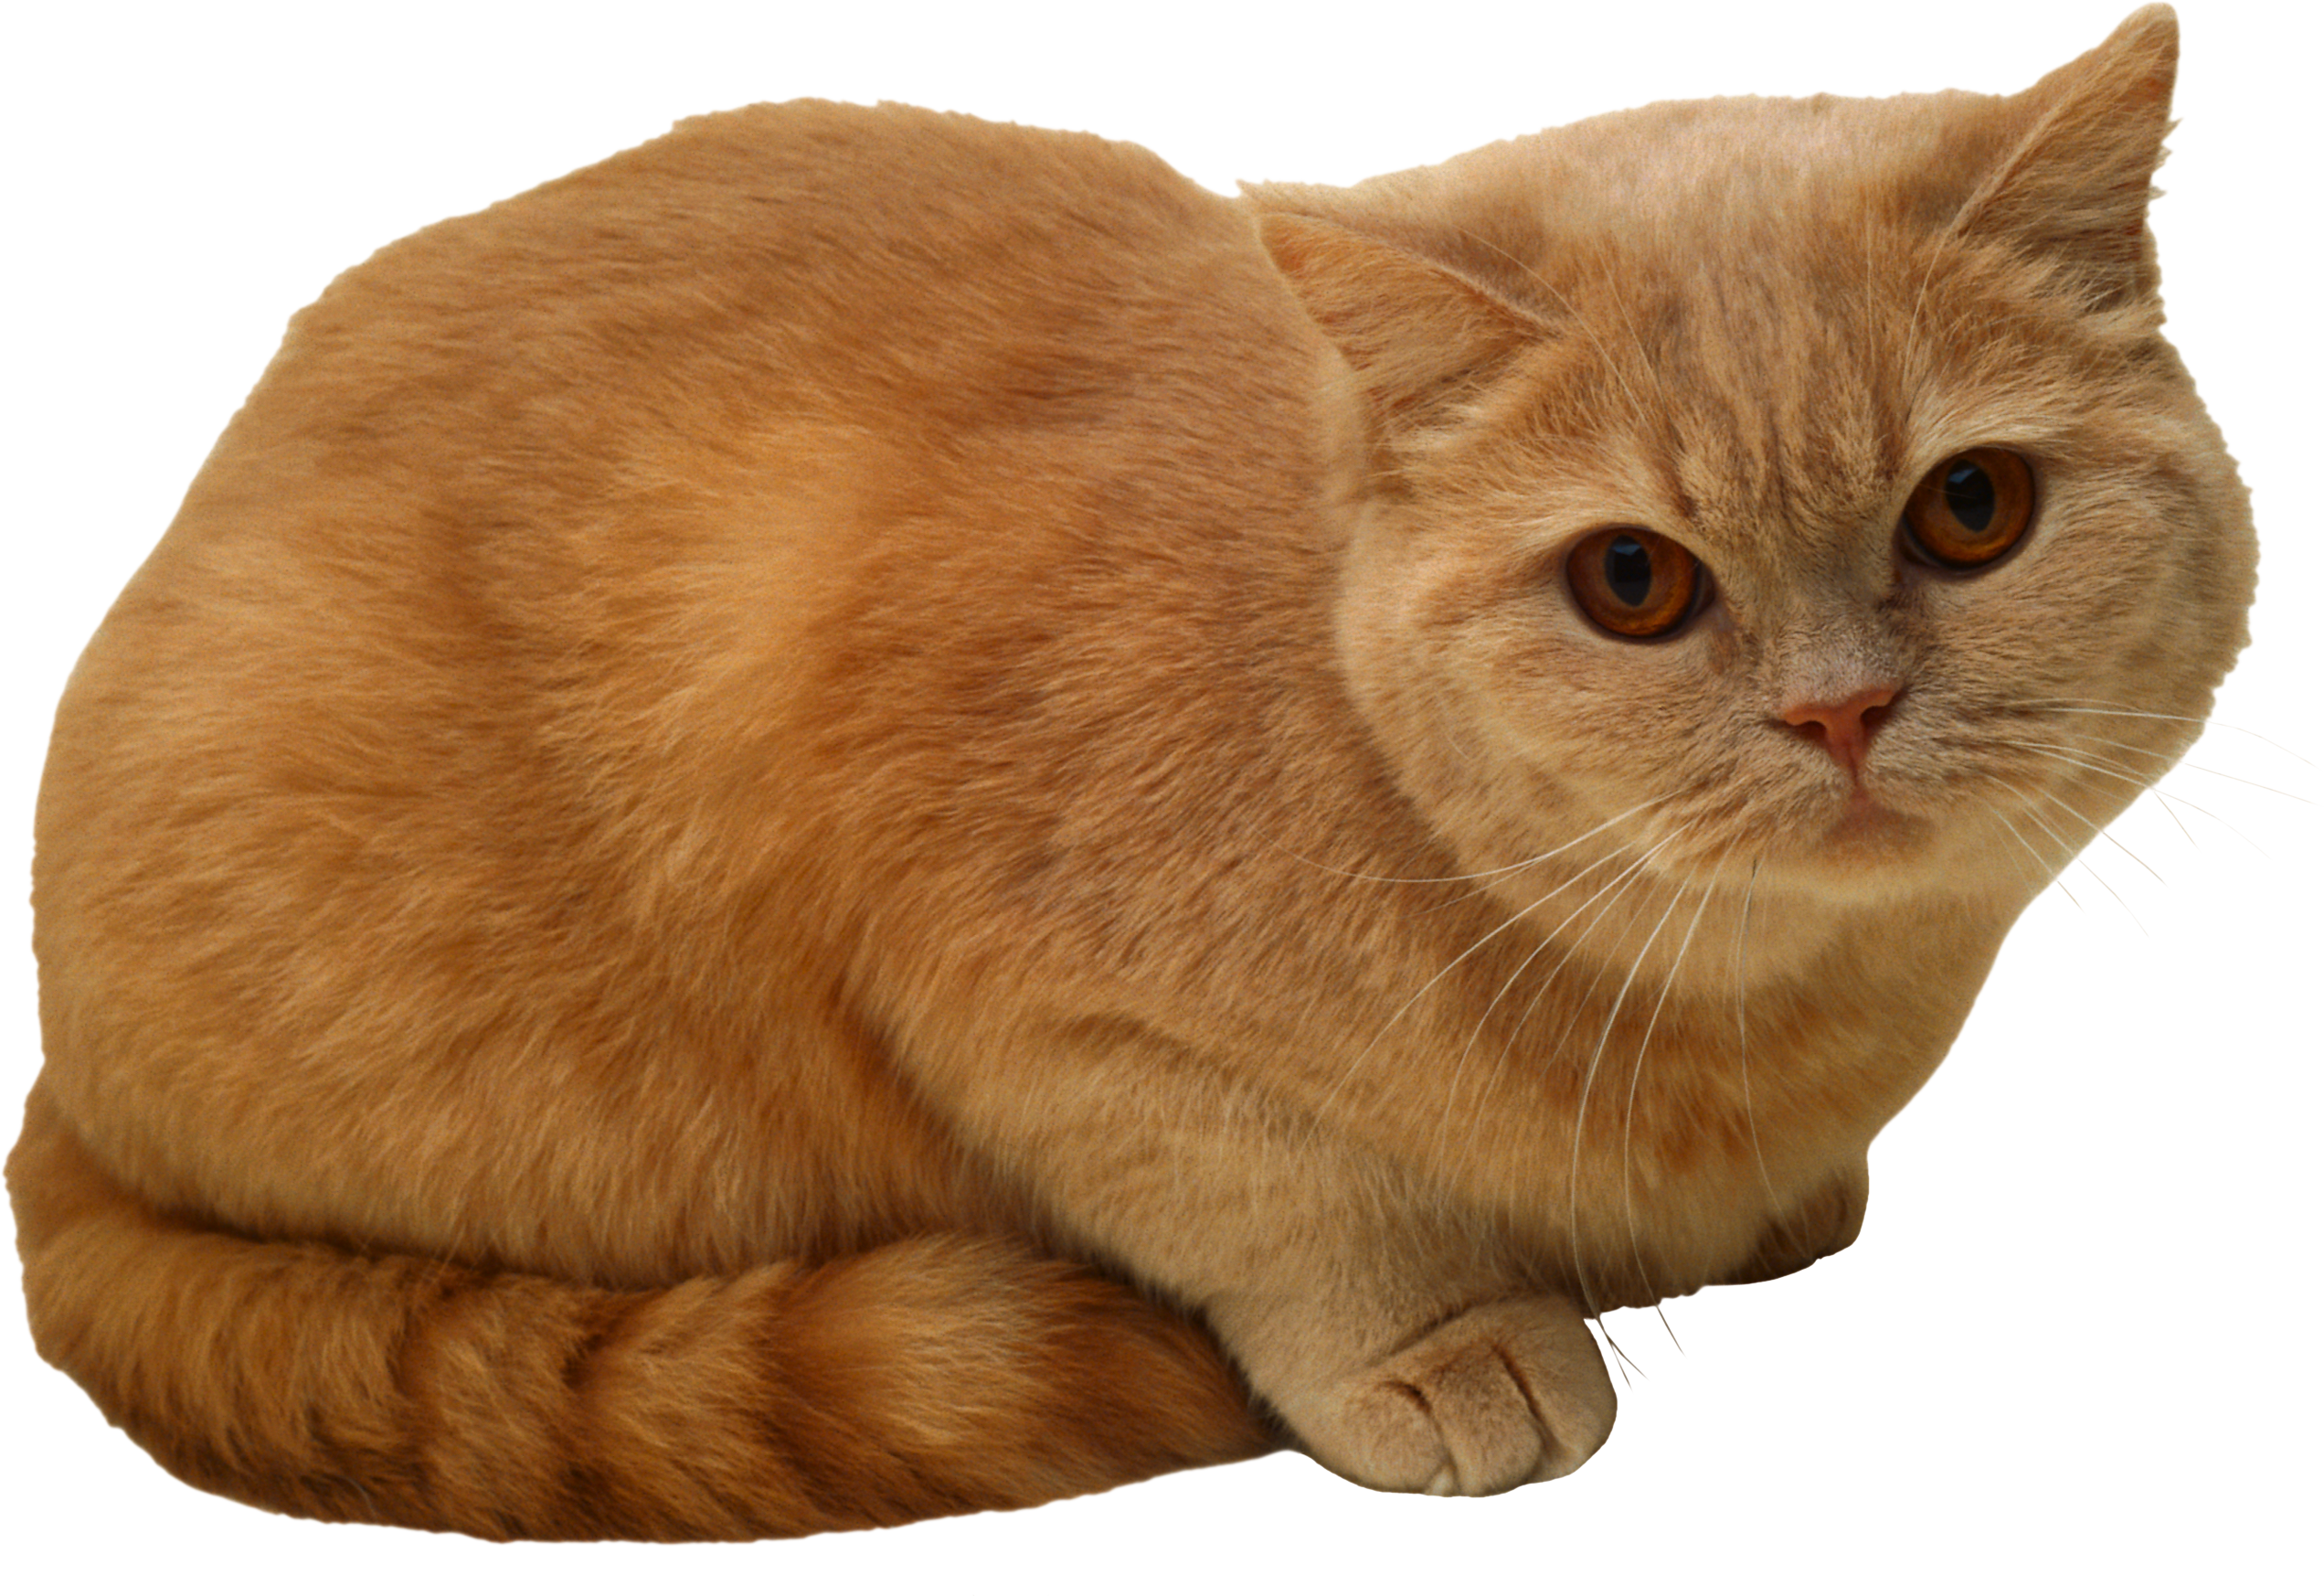
\includegraphics[width=.9\linewidth]{image/chat.png}
	\caption{Représentation d'un chat}
	\label{fig:chat1}
\end{figure}

\subsubsection{Partie 1.1.2}

\subparagraph{Partie 1.1.2.1}
~~\newline

\subparagraph{Partie 1.1.2.2}
~~\newline


\subsubsection{Partie 1.1.3 \label{sec:partie_1_1_3}}

\completeref{fig:chat3}

\bracompref{fig:chat3}

\begin{figure}[ht]
	\centering
	\begin{subfigure}[c]{0.45\textwidth}
		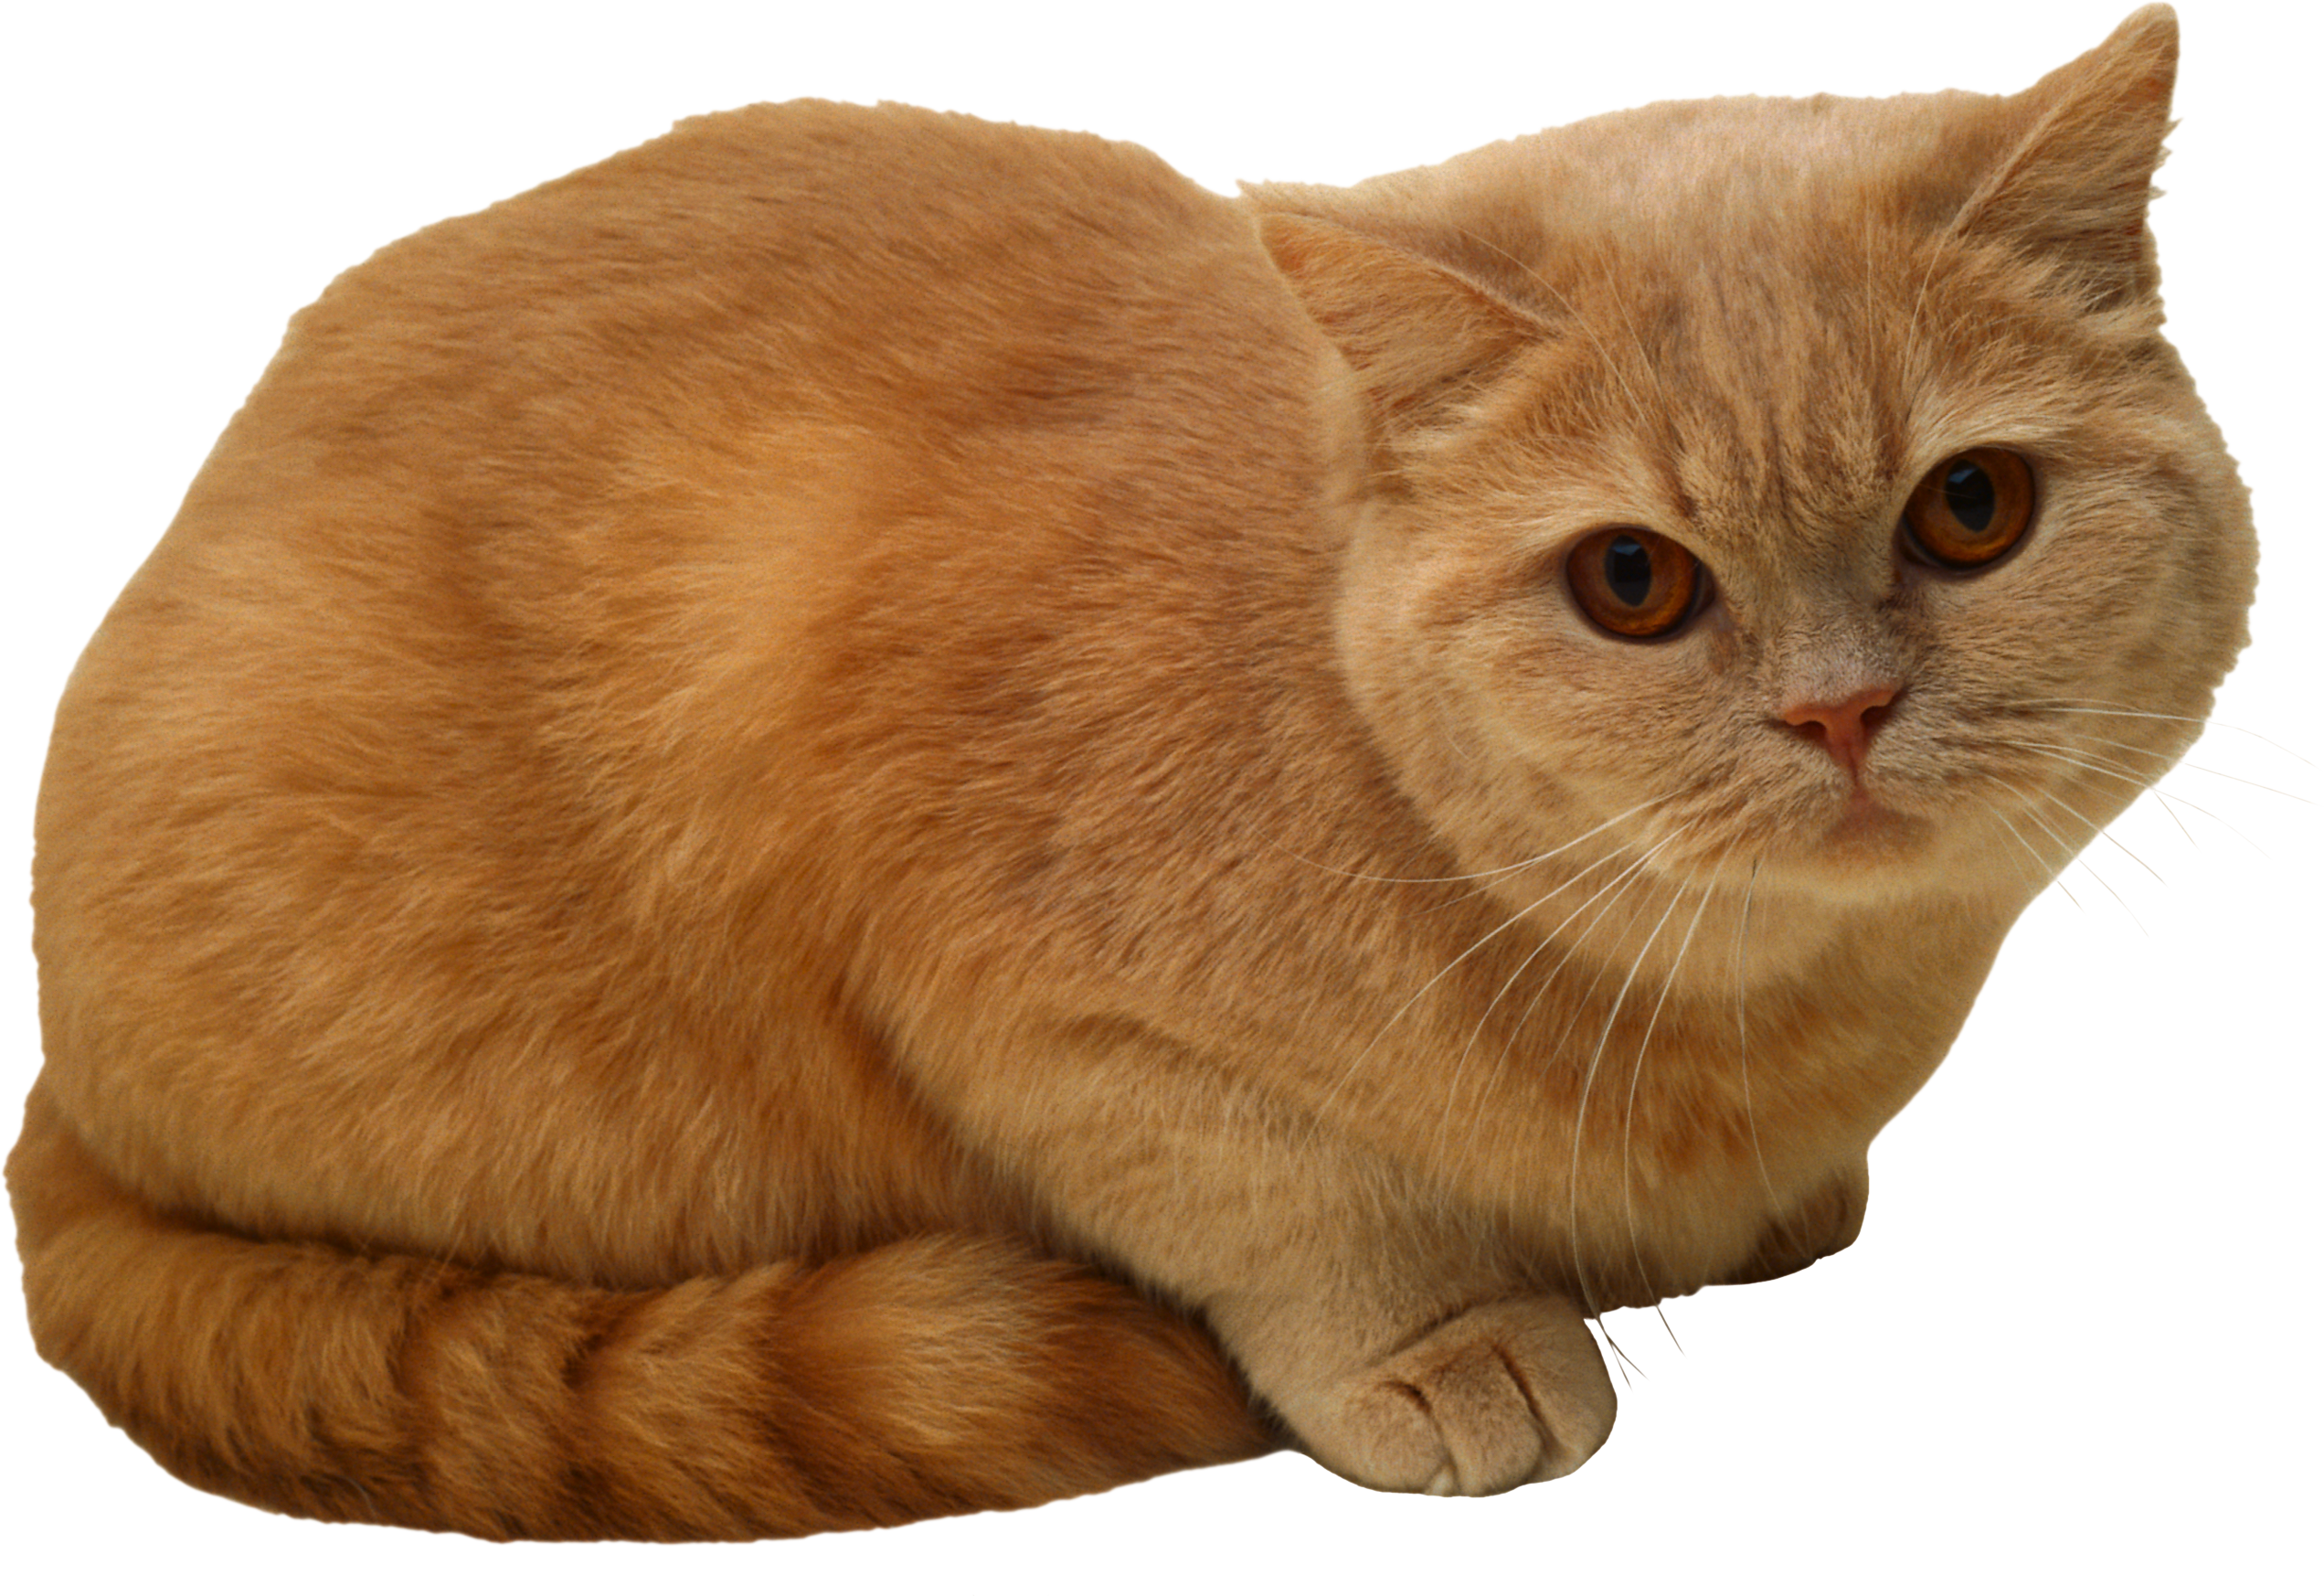
\includegraphics[width=\textwidth]{image/chat.png}
		\caption{Chat gauche}
	\end{subfigure}
	\hfill
	\begin{subfigure}[c]{0.45\textwidth}
		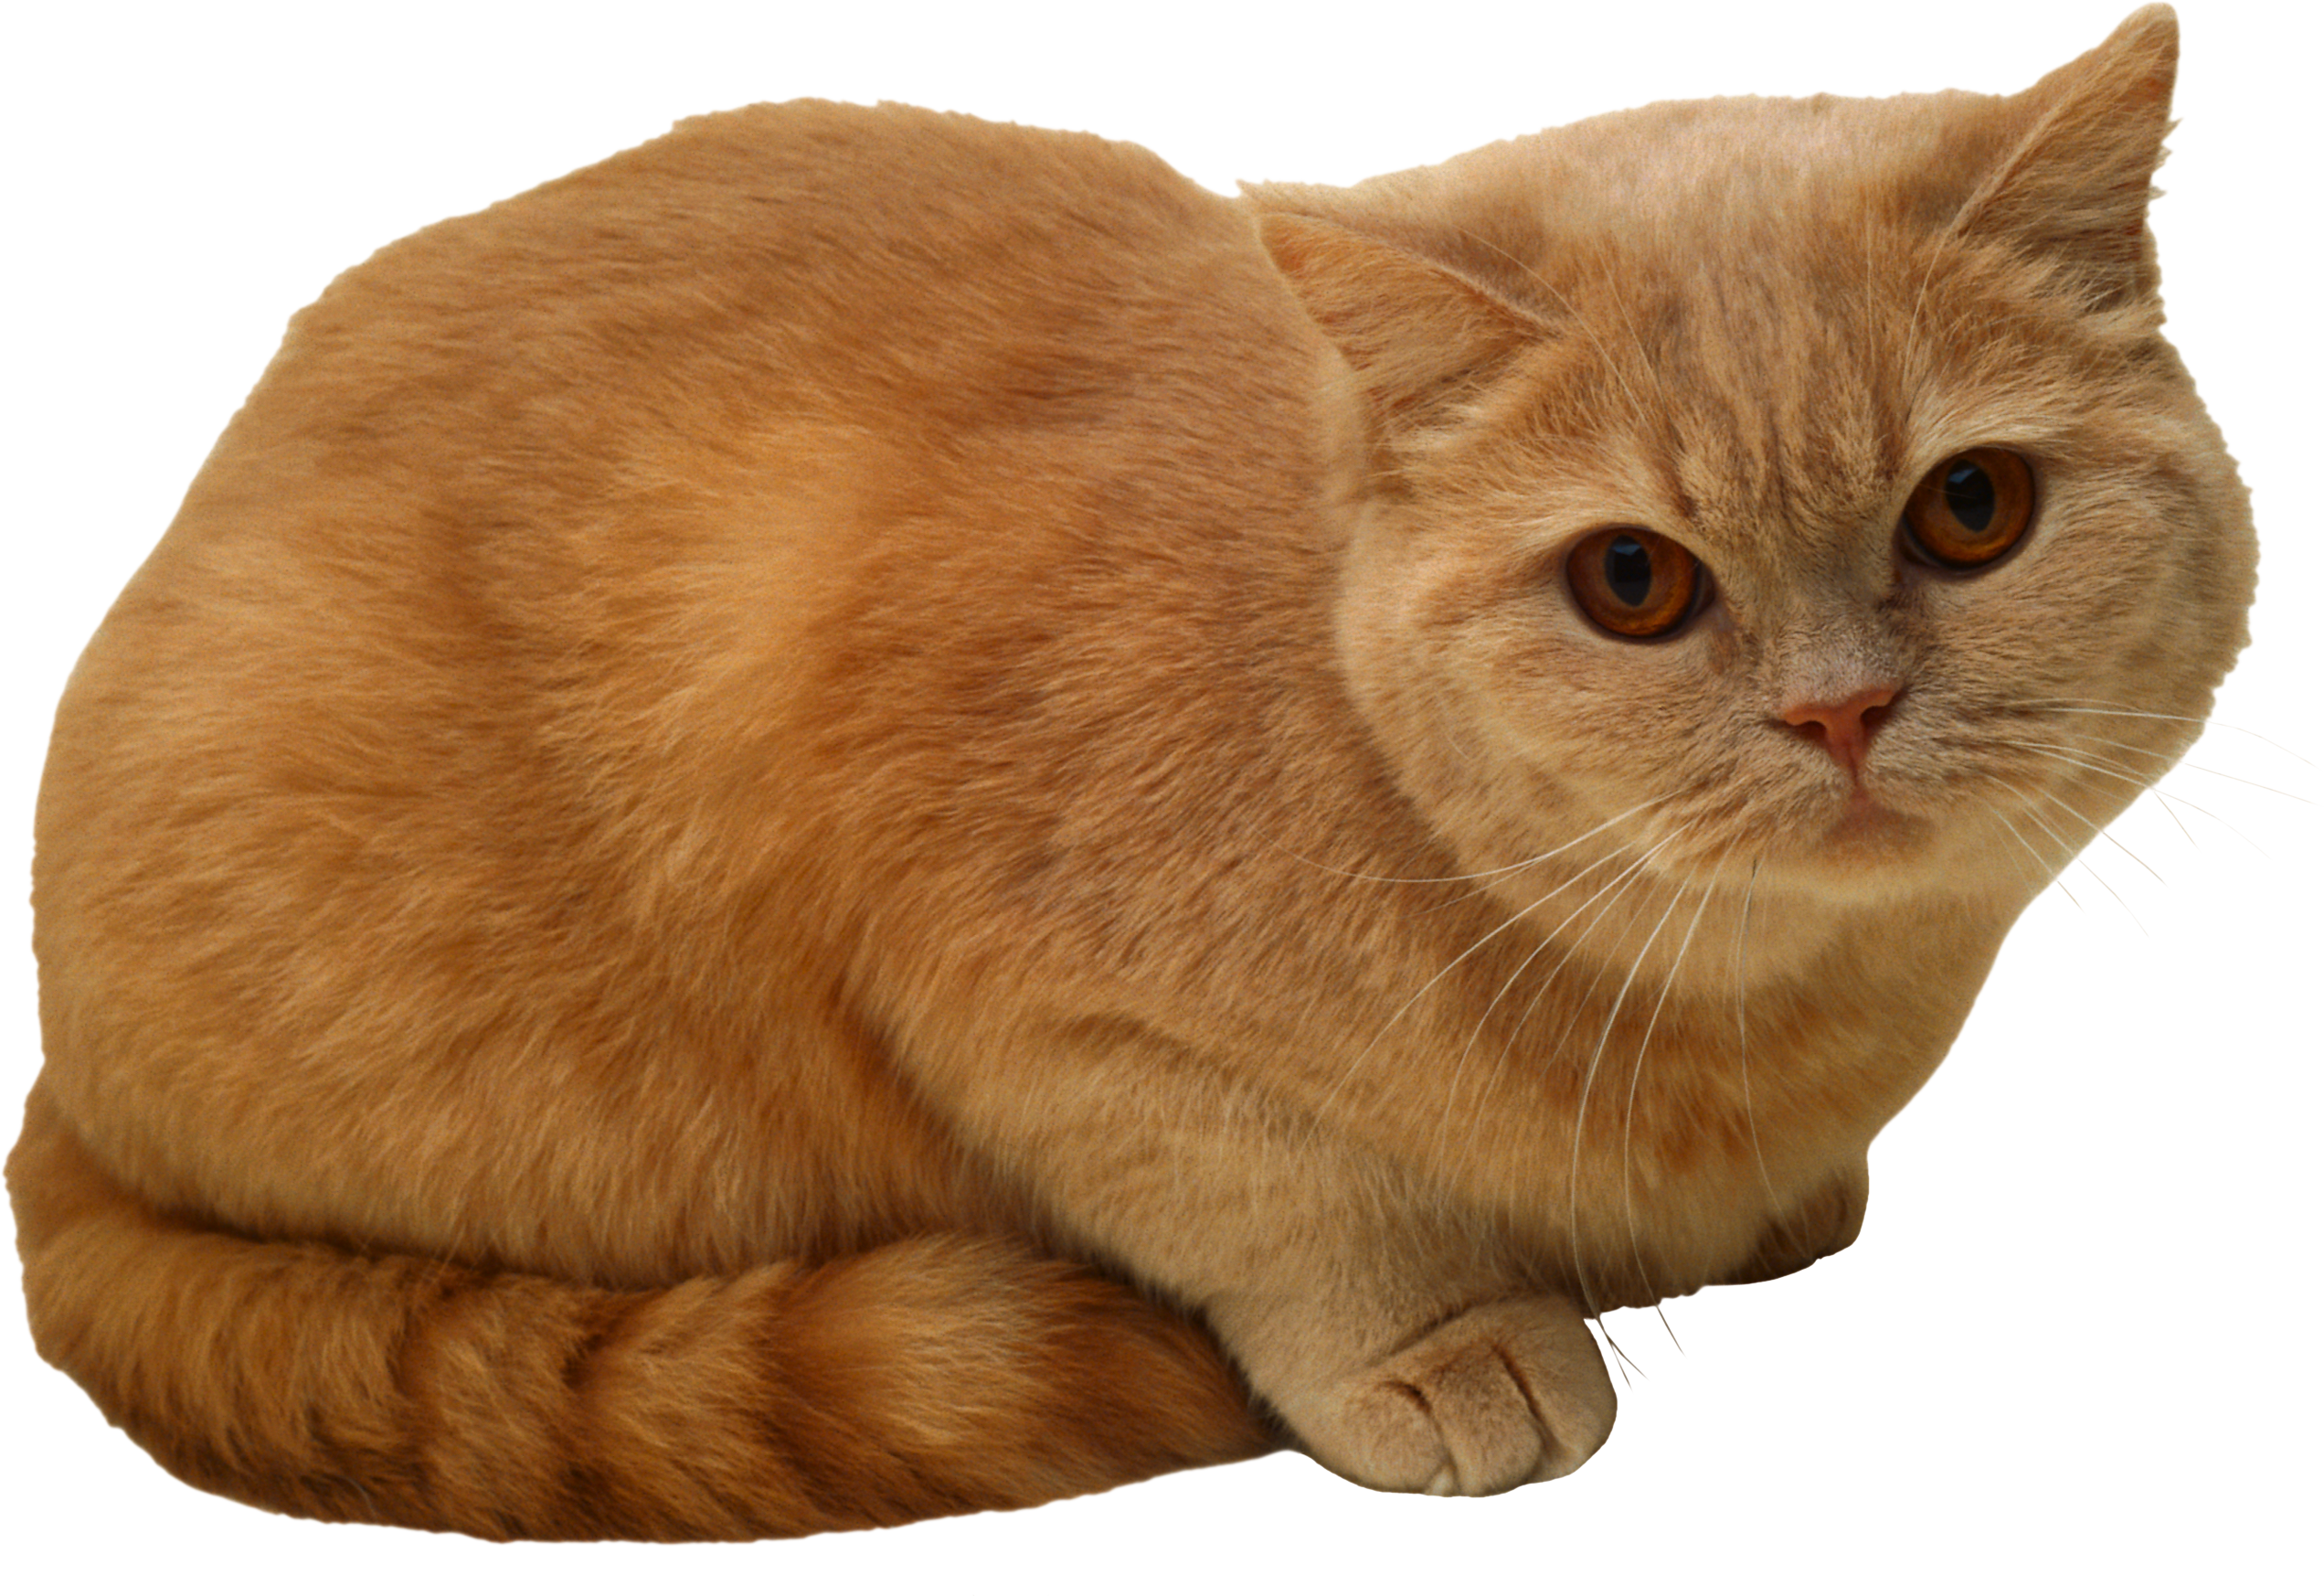
\includegraphics[width=\textwidth]{image/chat.png}
		\caption{Chat droite}
	\end{subfigure}
			
	\caption{Deux chats}
	\label{fig:chat3}
\end{figure}

\paragraph{Partie 1.1.3.1 \label{sec:partie_1_1_3_1}}
~~\newline

\paragraph{Partie 1.1.3.2}
\label{sec:partie_1_1_3_2}
~~\newline

Lien vers un titre : \Iref{sec:partie_1_1}

\subparagraph{Partie 1.1.3.2.1}
~~\newline

Acronyme full : \acrfull{epun}; Acronyme long : \acrlong{epun}; Acronyme short : \acrshort{epun}\newline

Note de bas de page\footnote{Note de base de page}\newline

Citation bibli : \cite{scikit-learn}, \cite{gnikit2022}, \cite{gnikit2022,scikit-learn}\newline

\begin{equation}
	y = f(\beta,X) + \varepsilon
	\label{eq:model}
\end{equation}

Lien vers l'équation : \ref{eq:model}

% Important : il ne faut pas que un code soit divisé entre deux page sinon il y a une erreur à la compile

\newpage
\autoref{el:vehicule}
\begin{lstlisting}[language=Python, caption=Définition de classe en Python, label=el:vehicule]
    class Vehicule:

        def __init__(self, marque, annee):
            self.marque = marque
            self.annee = annee

        def avancer(self):
            ...
\end{lstlisting}